\documentclass[10pt]{article}
\usepackage[usenames]{color} %used for font color
\usepackage{amssymb} %maths
\usepackage{amsmath} %maths
\usepackage[utf8]{inputenc} %useful to type directly diacritic characters
\usepackage{tkz-graph}
\usetikzlibrary{shapes,fit}\begin{document}
\[
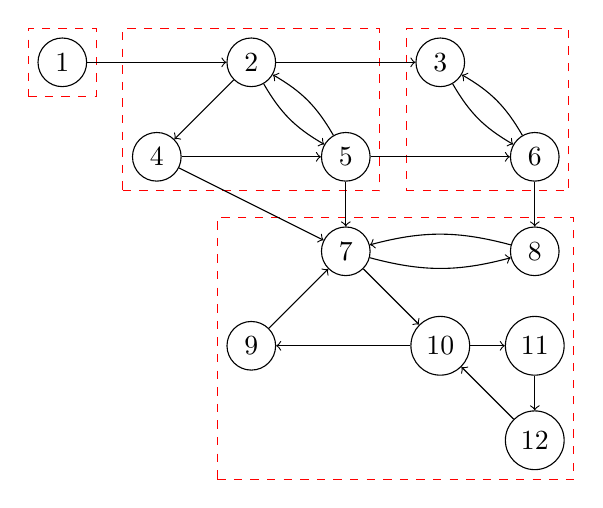
\begin{tikzpicture}[
block/.style={minimum width={width("99")}}]
  \node[shape=circle,draw=black] (1) at (0,0) {1};
  \node[shape=circle,draw=black] (2) at (2.4,0) {2};
  \node[shape=circle,draw=black] (3) at (4.8,0) {3};
  \node[shape=circle,draw=black] (4) at (1.2,-1.2) {4};
  \node[shape=circle,draw=black] (5) at (3.6,-1.2) {5};
  \node[shape=circle,draw=black] (6) at (6.0,-1.2) {6};
  \node[shape=circle,draw=black] (7) at (3.6,-2.4) {7};
  \node[shape=circle,draw=black] (8) at (6.0,-2.4) {8};
  \node[shape=circle,draw=black] (9) at (2.4,-3.6) {9};
  \node[shape=circle,draw=black] (10) at (4.8,-3.6) {10};
  \node[shape=circle,draw=black] (11) at (6.0,-3.6) {11};
  \node[shape=circle,draw=black] (12) at (6.0,-4.8) {12};

   \node[draw=red,dashed, fit=(1)](fit1) {};
   \node[draw=red,dashed, fit=(2) (4) (5)](fit2) {};
   \node[draw=red,dashed, fit=(3) (6)](fit3) {};
   \node[draw=red,dashed, fit=(7) (8) (9) (10) (11) (12) ](fit4) {};

  \path [->](1) edge node {} (2);
  \path [->](2) edge node {} (3);
  \path [->](2) edge node {} (4);
  \path [->](2) edge[bend right=15] node {} (5);
  \path [->](4) edge node {} (5);
  \path [->](5) edge[bend right=15] node {} (2);
  \path [->](3) edge[bend right=15] node {} (6);
  \path [->](6) edge[bend right=15] node {} (3);
  \path [->](5) edge node {} (6);
  \path [->](4) edge node {} (7);
  \path [->](5) edge node {} (7);
  \path [->](6) edge node {} (8);
  \path [->](7) edge[bend right=15] node {} (8);
  \path [->](8) edge[bend right=15] node {} (7);
  \path [->](9) edge node {} (7);
  \path [->](7) edge node {} (10);
  \path [->](10) edge node {} (9);
  \path [->](10) edge node {} (11);
  \path [->](11) edge node {} (12);
  \path [->](12) edge node {} (10);

\end{tikzpicture}\]
\end{document}